عملگر اتساع:
\begin{flalign*}
    A \oplus B = \bigcup_{b \in B} (A)_b = \{\, z \mid (\hat{B})_z \cap A \neq \varnothing \,\} &&
\end{flalign*}
عنصر ساختاری روی قطر اصلی، با مبدأ در مرکز، شامل سه نقطه است:
\begin{flalign*}
    B = \{(-1,-1),\,(0,0),\,(1,1)\}, \qquad \text{با مبدأ در } (0,0) &&
\end{flalign*}
چون هر پیکسل پیش‌زمینهٔ $A$ به ازای هر $b \in B$ یک‌بار جابه‌جا و کپی می‌شود، اتساع برابر اجتماع سه نسخهٔ شیفت‌یافتهٔ تصویر است:
\begin{flalign*}
    A \oplus B = A \;\cup\; (A)_{(-1,-1)} \;\cup\; (A)_{(1,1)} &&
\end{flalign*}
که در آن $(A)_{(-1,-1)}$ کل شکل را یک پیکسل به بالا-چپ و $(A)_{(1,1)}$ یک پیکسل به پایین-راست منتقل می‌کند؛ اجتماع این سه، شیء را در راستای قطر اصلی ضخیم‌تر می‌سازد و حفره‌های داخلی را در همان راستا کوچک می‌کند (نتیجهٔ نشان‌داده‌شده در شکل سمت راست).

تحلیل نتیجه:
\begin{flalign*}
    &\bullet\ \text{مرزها فقط در جهت قطری } \nearrow\!\!/\!\!\swarrow \text{ گسترش می‌یابند، نه به‌صورت همسان‌گرد.} \\
    &\bullet\ |A \oplus B| \geq |A| \quad (\text{چون } (0,0) \in B \Rightarrow A \subseteq A\oplus B). \\
    &\bullet\ \text{حفره‌ها و شکاف‌های نازک‌تر از پهنای } B \text{ در راستای قطر پر می‌شوند.} &&
\end{flalign*}

\LTR
\begin{center}
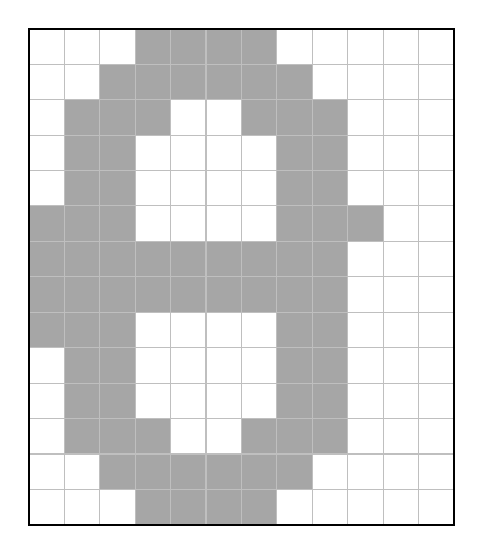
\begin{tikzpicture}[scale=0.45]
\def\N{12} % columns
\def\M{14} % rows
\draw[step=1, gray!50, thin] (0,0) grid (\N,\M);
\foreach \c/\r in {
  4/1,5/1,6/1,7/1,
  3/2,4/2,5/2,6/2,7/2,8/2,
  2/3,3/3,4/3,7/3,8/3,9/3,
  2/4,3/4,8/4,9/4,
  2/5,3/5,8/5,9/5,
  1/6,2/6,3/6,8/6,9/6,10/6,
  1/7,2/7,3/7,4/7,5/7,6/7,7/7,8/7,9/7,
  1/8,2/8,3/8,4/8,5/8,6/8,7/8,8/8,9/8,
  1/9,2/9,3/9,8/9,9/9,
  2/10,3/10,8/10,9/10,
  2/11,3/11,8/11,9/11,
  2/12,3/12,4/12,7/12,8/12,9/12,
  3/13,4/13,5/13,6/13,7/13,8/13,
  4/14,5/14,6/14,7/14
}{
  \fill[gray!70] (\c-1, \M-\r) rectangle (\c, \M-\r+1);
}
\draw[step=1, gray!50, thin] (0,0) grid (\N,\M);
\draw[black, thick] (0,0) rectangle (\N,\M);
\end{tikzpicture}
\end{center}
\RTL

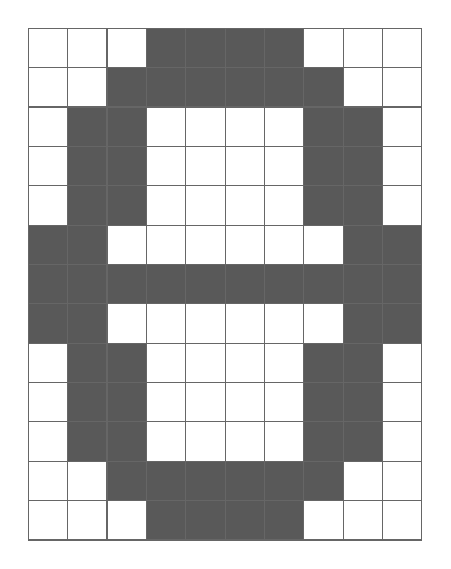
\begin{tikzpicture}[x=0.5cm, y=0.5cm]
    % Define colors to match the image
    \colorlet{gridcolor}{black!60}
    \colorlet{fillcolor}{black!65}

    % Fill the dark squares (grouped logically by section)
    \fill[fillcolor]
        % --- Top Loop ---
        % Top edge (Width 4)
        (3,12) rectangle (7,13)
        % Row 2 step out (Width 6)
        (2,11) rectangle (8,12)
        % Upper vertical side bars (Height 3)
        (1,8)  rectangle (3,11)
        (7,8)  rectangle (9,11)
        
        % --- Middle Section ---
        % Left ear (Height 3, Width 2)
        (0,5)  rectangle (2,8)
        % Right ear (Height 3, Width 2)
        (8,5)  rectangle (10,8)
        % Middle crossbar connecting the ears (Width 6, Height 1)
        (2,6)  rectangle (8,7)
        
        % --- Bottom Loop ---
        % Lower vertical side bars (Height 3)
        (1,2)  rectangle (3,5)
        (7,2)  rectangle (9,5)
        % Row 12 step in (Width 6)
        (2,1)  rectangle (8,2)
        % Bottom edge (Width 4)
        (3,0)  rectangle (7,1);

    % Draw the 10x13 grid on top
    \draw[step=1, gridcolor, thin] (0,0) grid (10,13);
\end{tikzpicture}

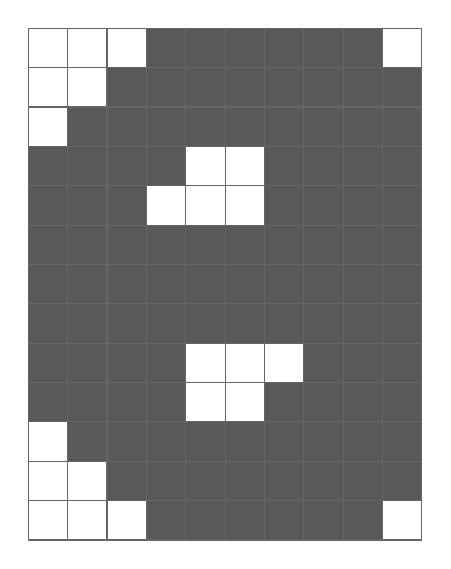
\begin{tikzpicture}[x=0.5cm, y=0.5cm]
    \colorlet{gridcolor}{black!60}
    \colorlet{fillcolor}{black!65}

    \fill[fillcolor]
        % Bottom edge region (y=0..1)
        (3,0) rectangle (9,1)
        % y=1..2
        (2,1) rectangle (10,2)
        % y=2..3
        (1,2) rectangle (10,3)
        % y=3..4
        (0,3) rectangle (4,4) (6,3) rectangle (10,4)
        % y=4..5
        (0,4) rectangle (4,5) (7,4) rectangle (10,5)
        % y=5..6 (middle band)
        (0,5) rectangle (10,6)
        % y=6..7
        (0,6) rectangle (10,7)
        % y=7..8
        (0,7) rectangle (10,8)
        % y=8..9
        (0,8) rectangle (3,9) (6,8) rectangle (10,9)
        % y=9..10
        (0,9) rectangle (4,10) (6,9) rectangle (10,10)
        % y=10..11
        (1,10) rectangle (10,11)
        % y=11..12
        (2,11) rectangle (10,12)
        % y=12..13 (top edge)
        (3,12) rectangle (9,13);

    \draw[step=1, gridcolor, thin] (0,0) grid (10,13);
\end{tikzpicture}

\LTR
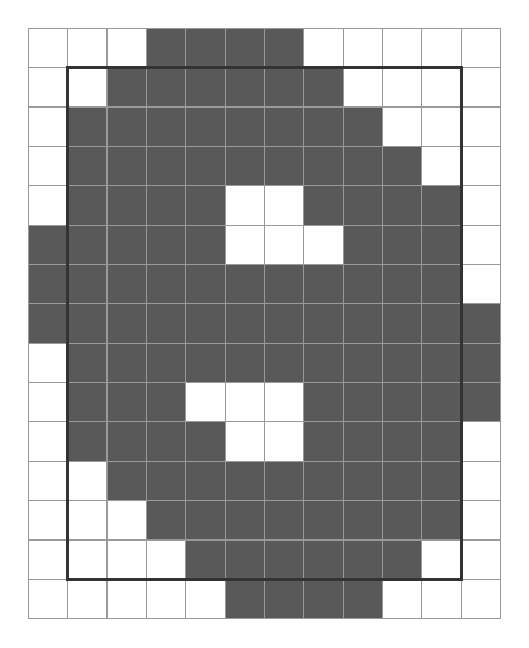
\begin{tikzpicture}[x=0.5cm, y=0.5cm]
    % Define colors
    \colorlet{gridcolor}{black!40}
    \colorlet{fillcolor}{black!65}
    \colorlet{origbox}{black!80}

    % Fill the newly dilated shape
    % Note: The coordinates extend from x=-1 to 10 and y=-1 to 13
    \fill[fillcolor]
        % y=13 (Expanded top)
        (2,13) rectangle (6,14)
        % y=12
        (1,12) rectangle (7,13)
        % y=11
        (0,11) rectangle (8,12)
        % y=10
        (0,10) rectangle (9,11)
        % y=9
        (0,9)  rectangle (4,10)
        (6,9)  rectangle (10,10)
        % y=8
        (-1,8) rectangle (4,9)
        (7,8)  rectangle (10,9)
        % y=7
        (-1,7) rectangle (10,8)
        % y=6 (Expanded crossbar)
        (-1,6) rectangle (11,7)
        % y=5
        (0,5)  rectangle (11,6)
        % y=4
        (0,4)  rectangle (3,5)
        (6,4)  rectangle (11,5)
        % y=3
        (0,3)  rectangle (4,4)
        (6,3)  rectangle (10,4)
        % y=2
        (1,2)  rectangle (10,3)
        % y=1
        (2,1)  rectangle (10,2)
        % y=0
        (3,0)  rectangle (9,1)
        % y=-1 (Expanded bottom)
        (4,-1) rectangle (8,0);

    % Draw the expanded bounding grid (-1 to 11 in X, -1 to 14 in Y)
    \draw[step=1, gridcolor, thin] (-1,-1) grid (11,14);

    % Draw a thicker boundary for the original 10x13 grid to show context
    \draw[origbox, very thick] (0,0) rectangle (10,13);

\end{tikzpicture}
\RTL

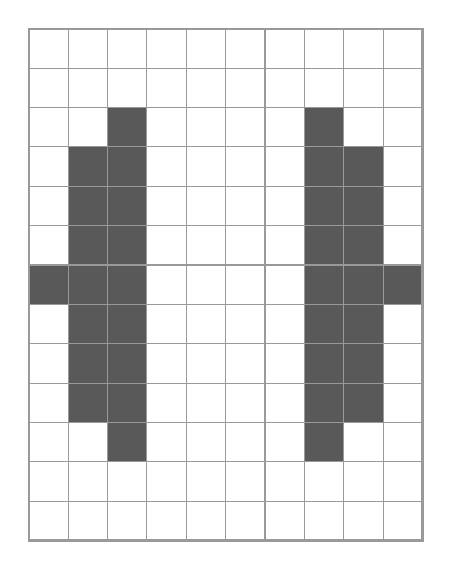
\begin{tikzpicture}[x=0.5cm, y=0.5cm]
    % Define colors
    \colorlet{gridcolor}{black!40}
    \colorlet{fillcolor}{black!65}

    % Fill the eroded shape
    \fill[fillcolor]
        % --- Left vertical section ---
        % Tip of the left ear (originally 3 pixels tall, reduced to 1)
        (0,6) rectangle (1,7)
        % Middle column of left bar (originally 9 tall, reduced to 7)
        (1,3) rectangle (2,10)
        % Inner column of left bar (originally 11 tall, reduced to 9)
        (2,2) rectangle (3,11)
        
        % --- Right vertical section ---
        % Inner column of right bar (originally 11 tall, reduced to 9)
        (7,2) rectangle (8,11)
        % Middle column of right bar (originally 9 tall, reduced to 7)
        (8,3) rectangle (9,10)
        % Tip of the right ear (originally 3 pixels tall, reduced to 1)
        (9,6) rectangle (10,7);

    % Draw the 10x13 grid
    \draw[step=1, gridcolor, thin] (0,0) grid (10,13);

    % Draw a thicker boundary for the grid
    \draw[gridcolor, thick] (0,0) rectangle (10,13);

\end{tikzpicture}